\documentclass[a4paper,12pt]{article}
\usepackage{amsmath,amsfonts,amsthm,amssymb, mathtools,steinmetz, gensymb, siunitx}	% LOADS USEFUL MATH STUFF
\usepackage{xcolor,graphicx}
\usepackage[margin=0.5in,a4paper]{geometry} 				% ADJUSTS PAGE
\usepackage{setspace}
\usepackage{caption}
\usepackage{tikz}
\usepackage{pgf,tikz,pgfplots}
\usepackage{mathrsfs}
\usepackage{fancyhdr}
\usepackage{float}
\usepackage{array}

\usetikzlibrary{decorations.pathreplacing,decorations.markings, arrows.meta}

\newcommand{\defeq}{\vcentcolon=}
\newcommand\block[1]{\hspace*{#1}}
\newcommand{\rpm}{\sbox0{$1$}\sbox2{$\scriptstyle\pm$}
	  \raise\dimexpr(\ht0-\ht2)/2\relax\box2 }
	  
\newlength{\QNo}
\settowidth{\QNo}{2.}

\newlength{\QLetter}
\settowidth{\QLetter}{(a)}

\pagestyle{fancy}
\rhead{Partial Differential Equations Tutorial}
\lhead{J L Gouws}

\begin{document}
\thispagestyle{empty}

{\Large \textbf{Numerical Modelling Assignment 2}} \hfill {\Large \textbf{J L Gouws}}\\
\block{1.0cm} {\large \textbf{\today}} \hfill {\large \textbf{19G4436}}\\
\begin{figure}[!h]
  \centering
  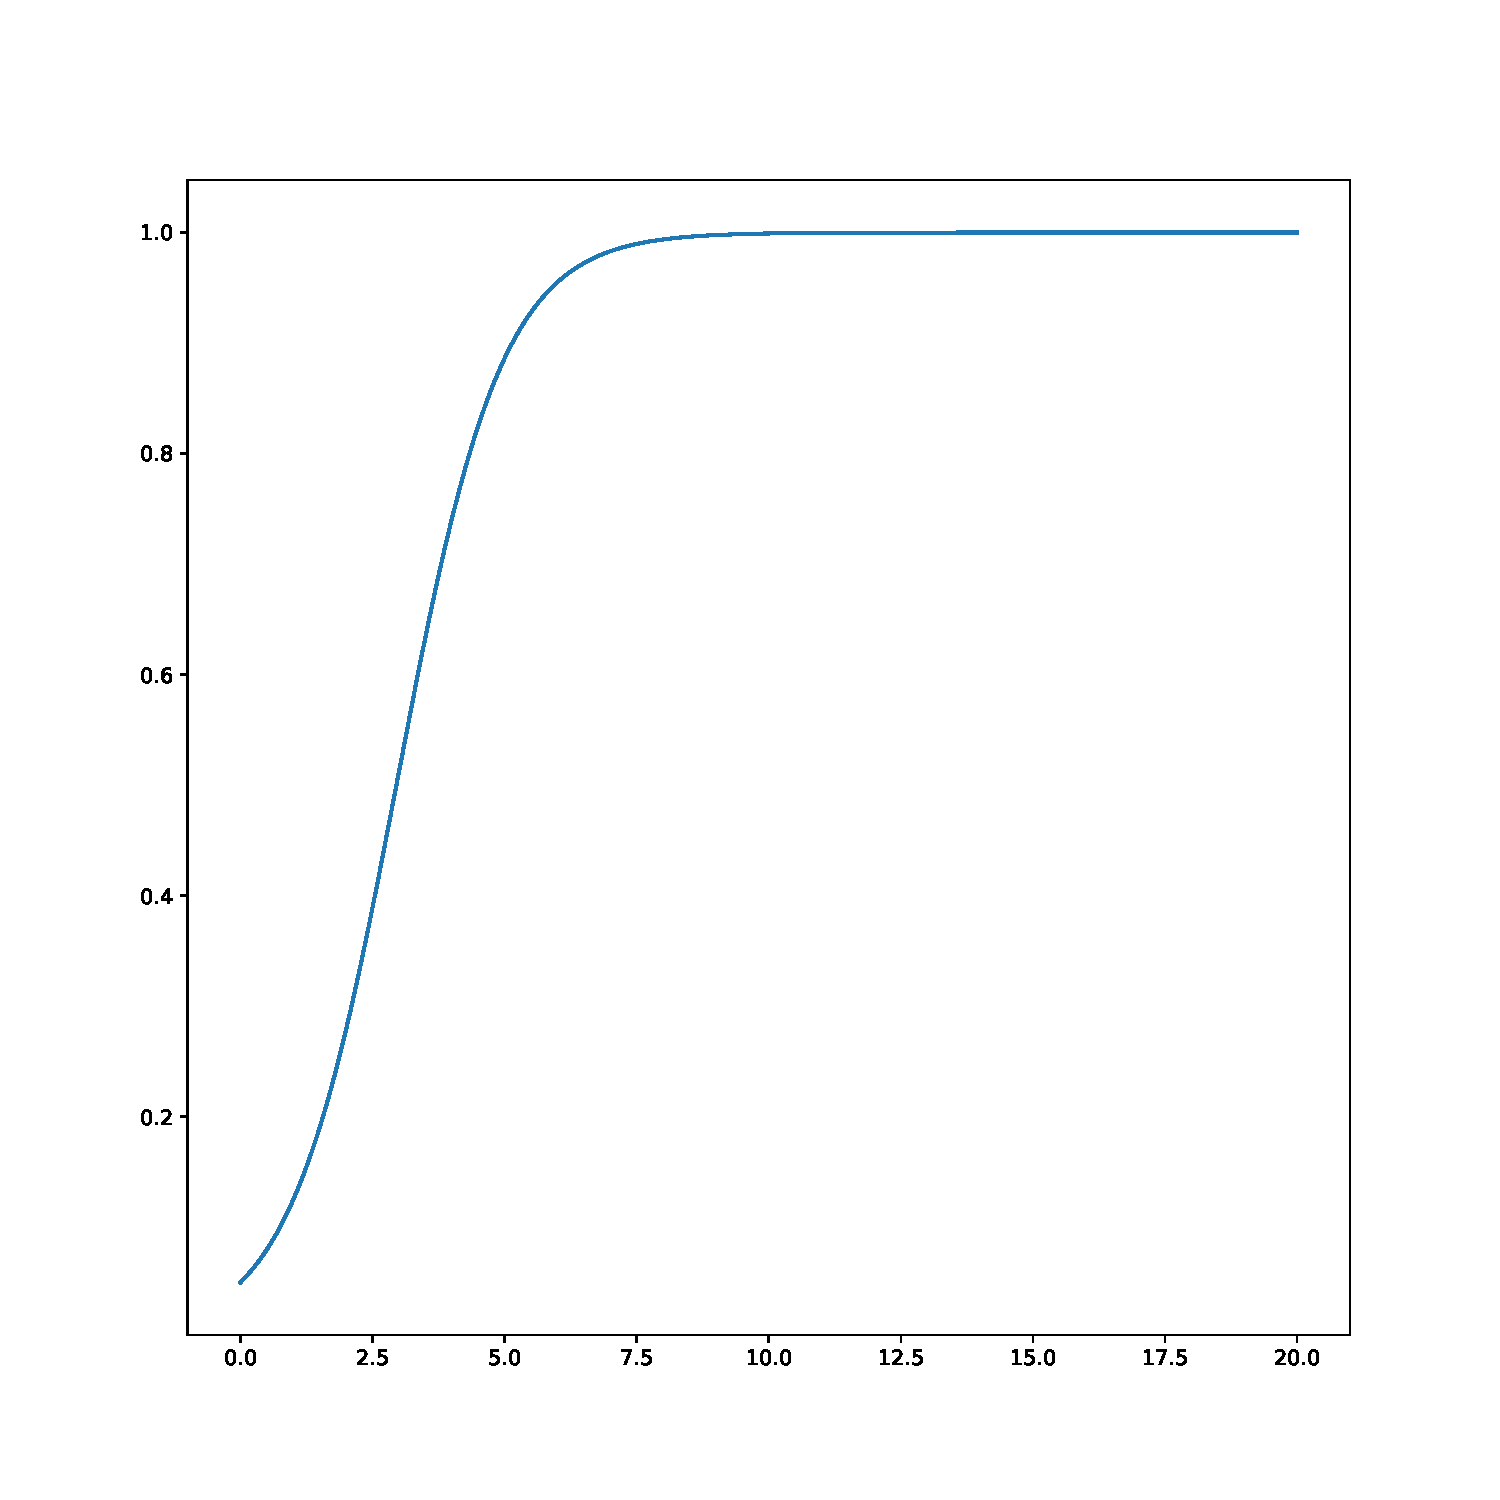
\includegraphics[scale = 0.5]{1a.pdf}
  \caption{The Euler Method Solution of the Logistic Equation}
  \label{fig:eulerLogistic}
\end{figure}

\begin{figure}[!h]
  \centering
  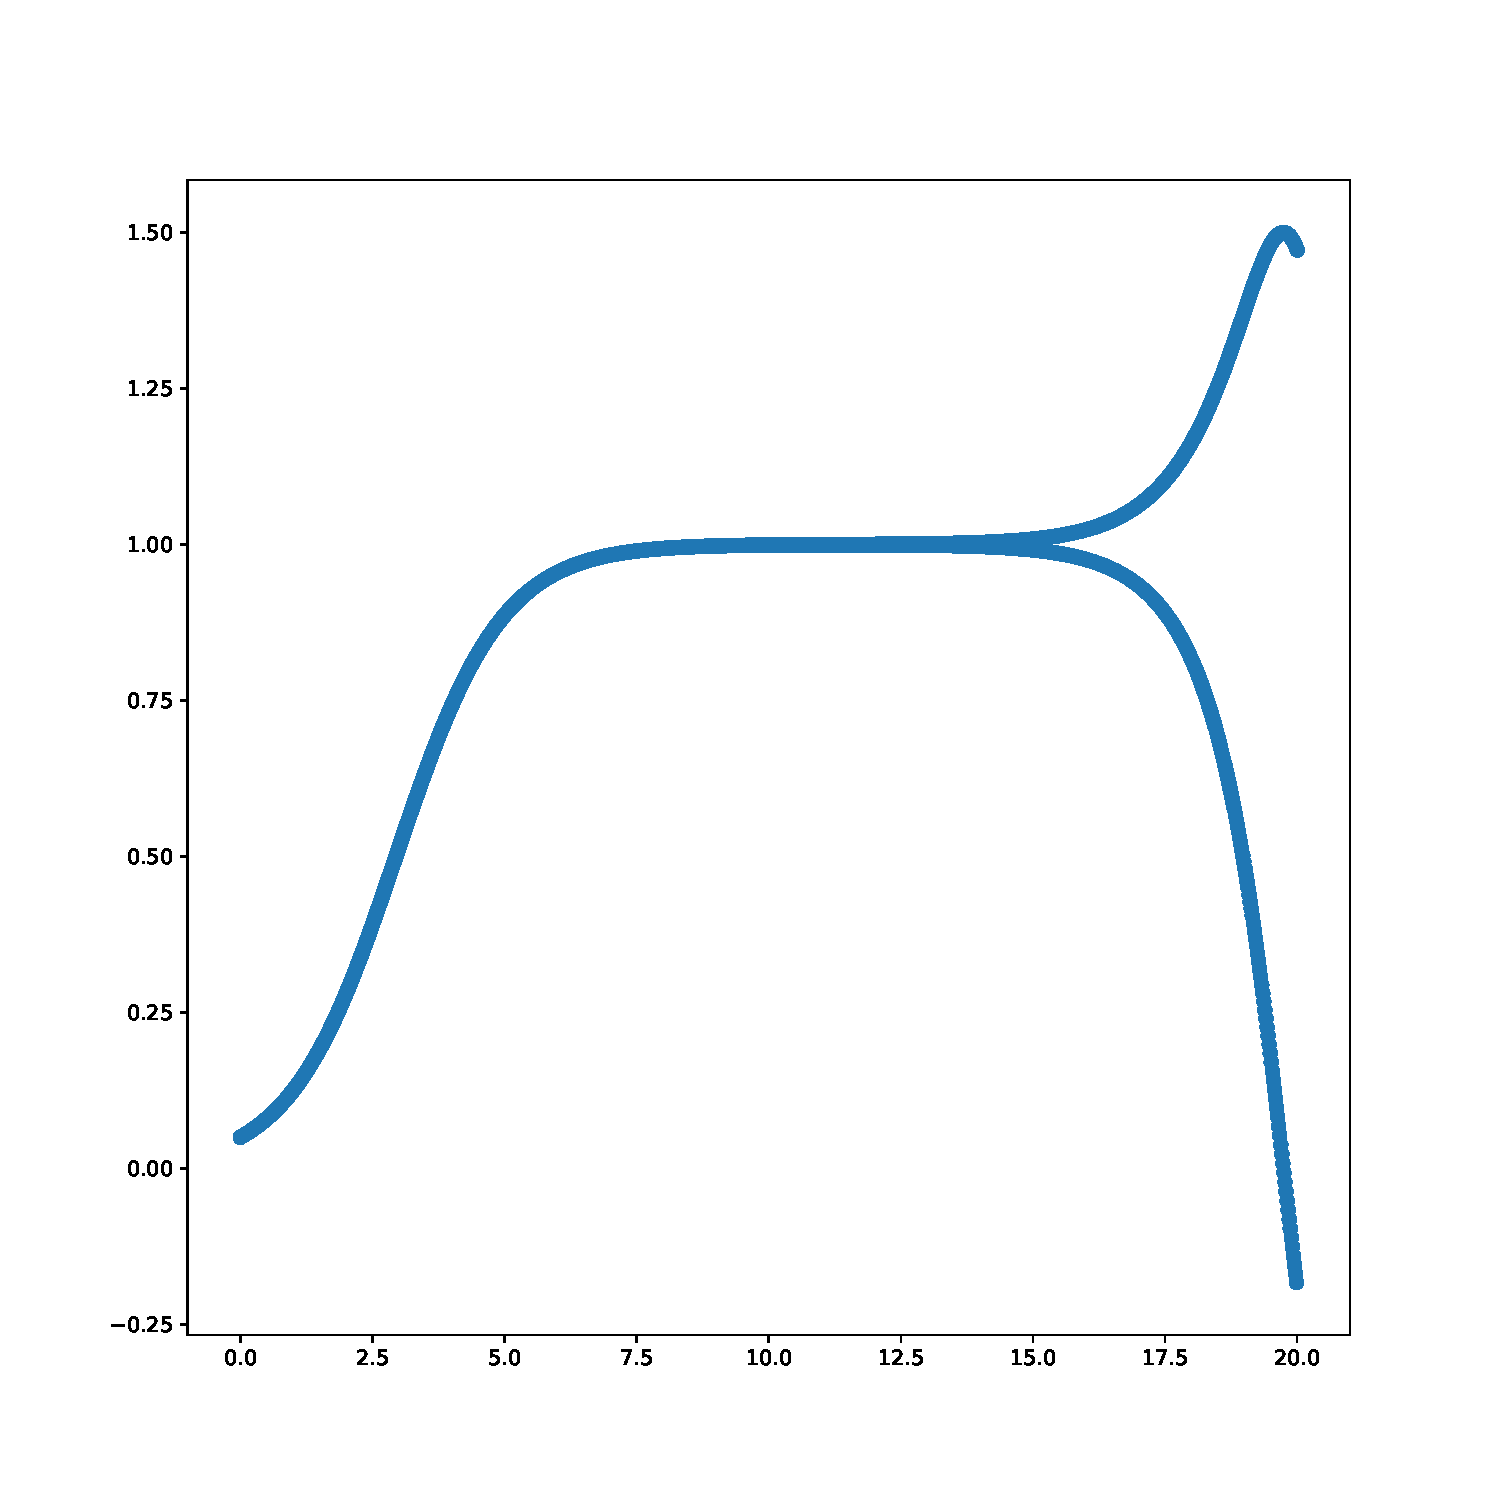
\includegraphics[scale = 0.5]{1b.pdf}
  \caption{The Midpoint Method Solution of the Logistic Equation}
  \label{fig:eulerLogistic}
\end{figure}

\begin{figure}[!h]
  \centering
  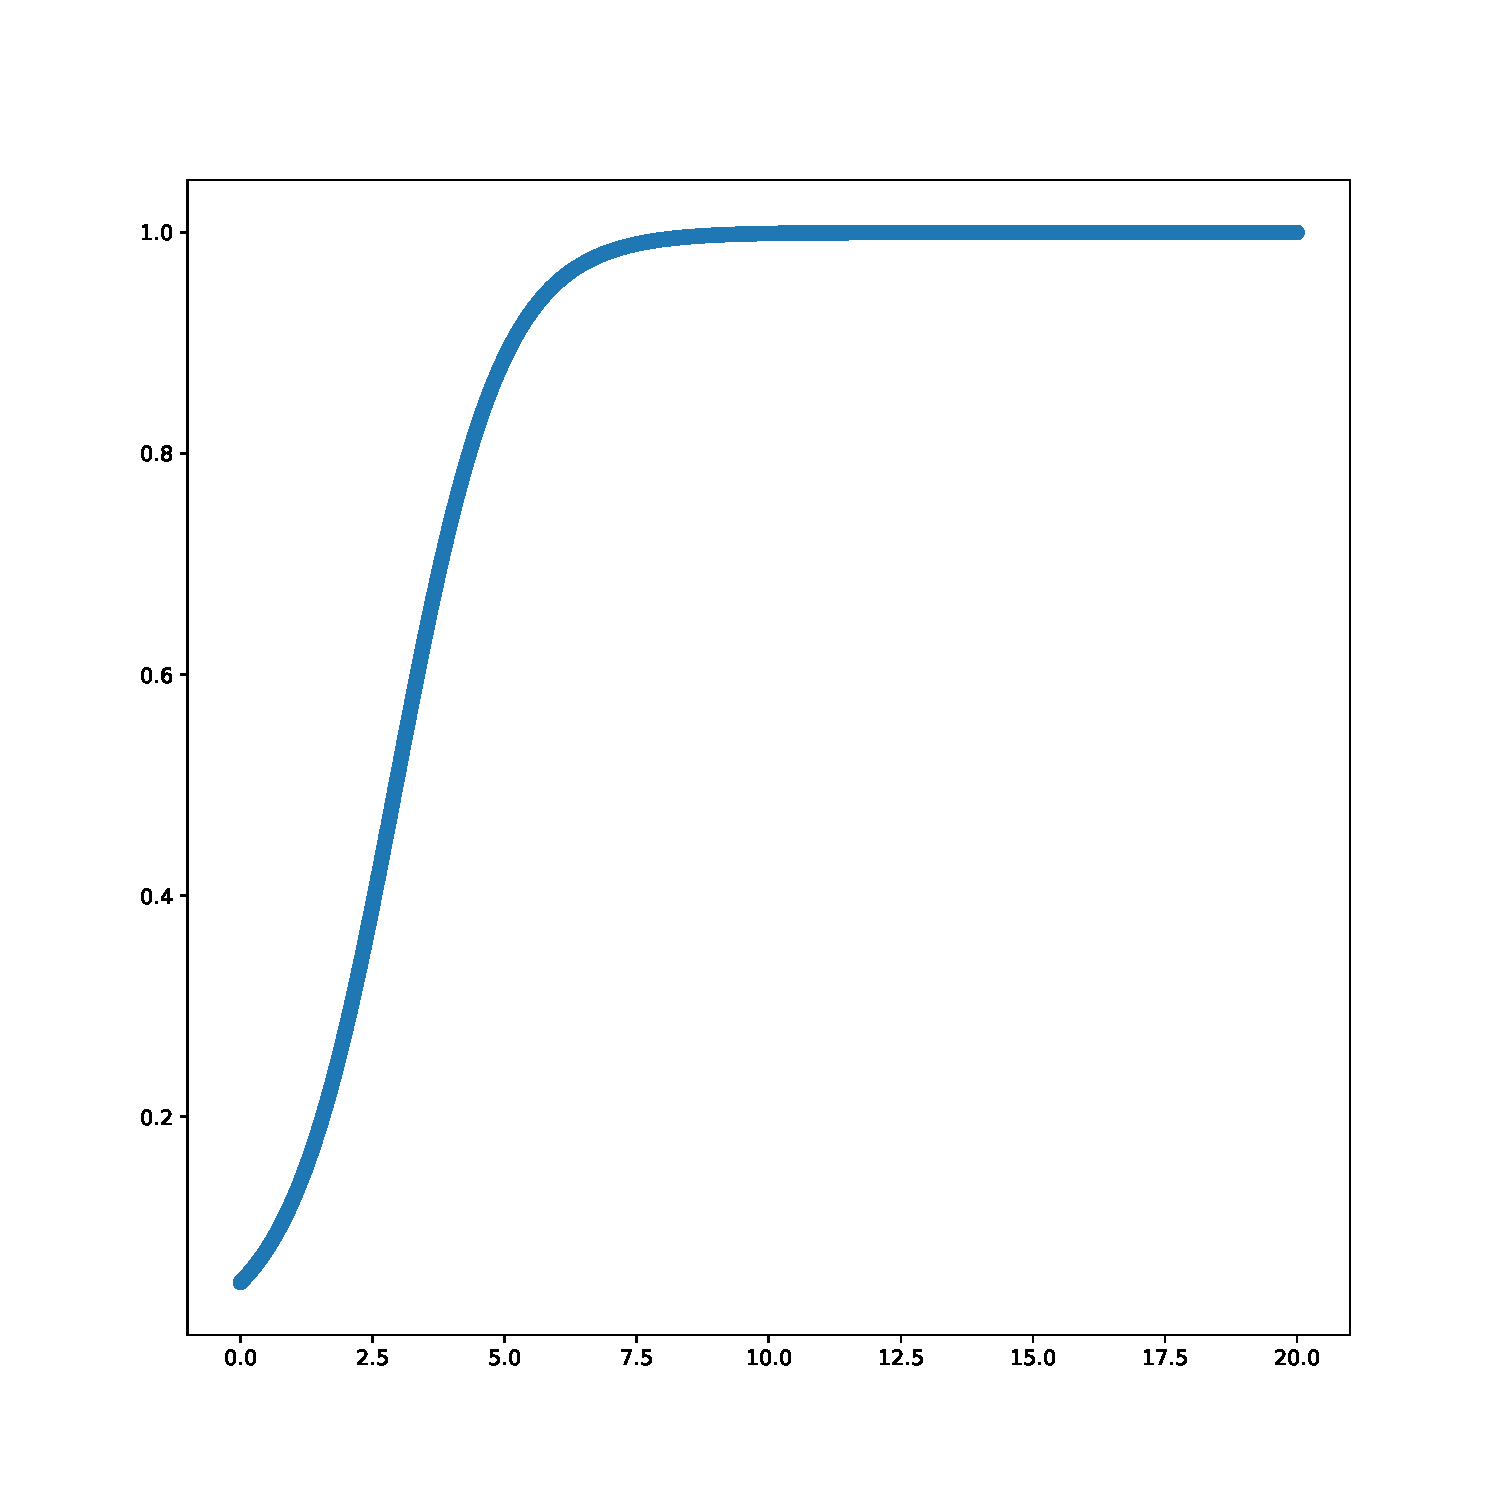
\includegraphics[scale = 0.5]{1c.pdf}
  \caption{A Second Order Runge Kutta Method Solution of the Logistic Equation}
  \label{fig:eulerLogistic}
\end{figure}

\begin{figure}[!h]
  \centering
  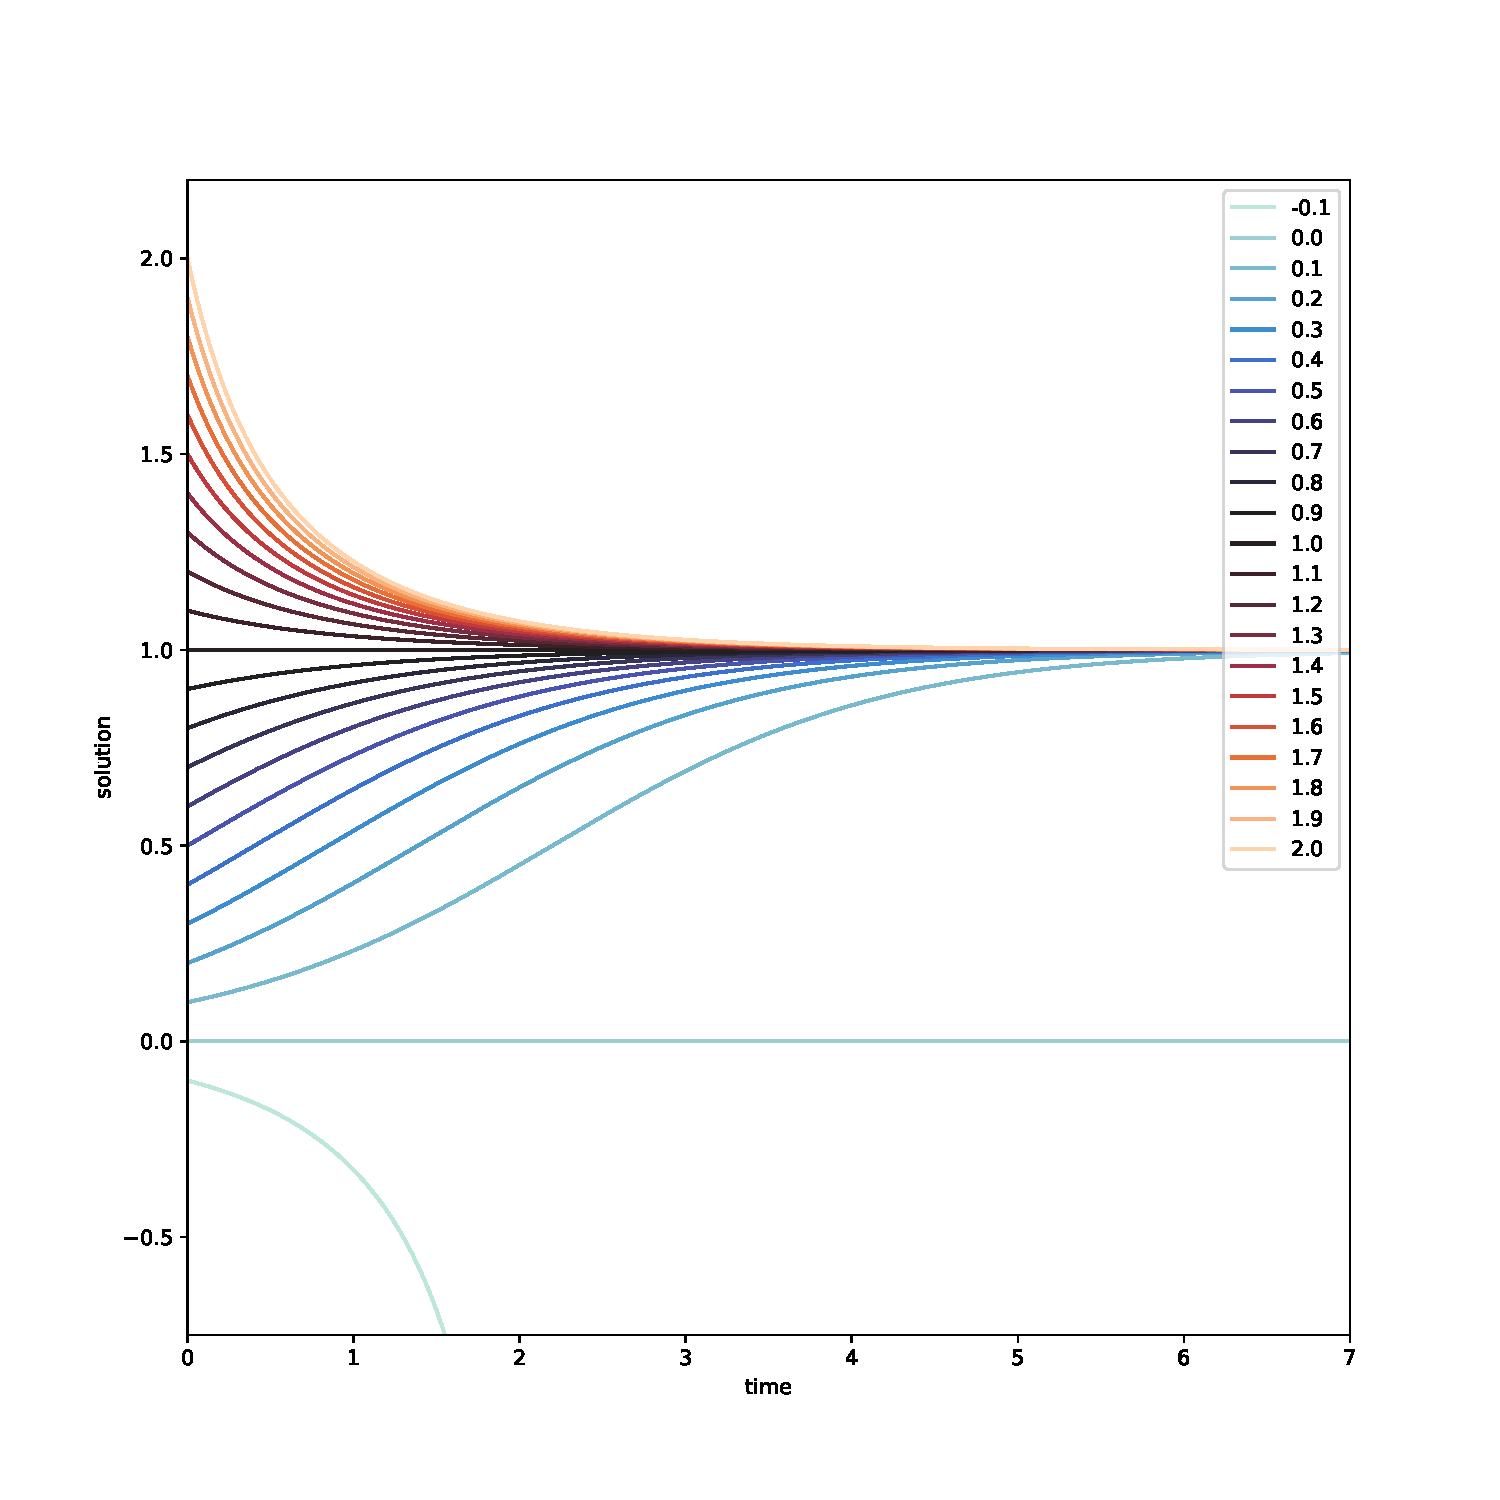
\includegraphics[scale = 0.75]{2.pdf}
\end{figure}

\begin{figure}[!h]
  \centering
  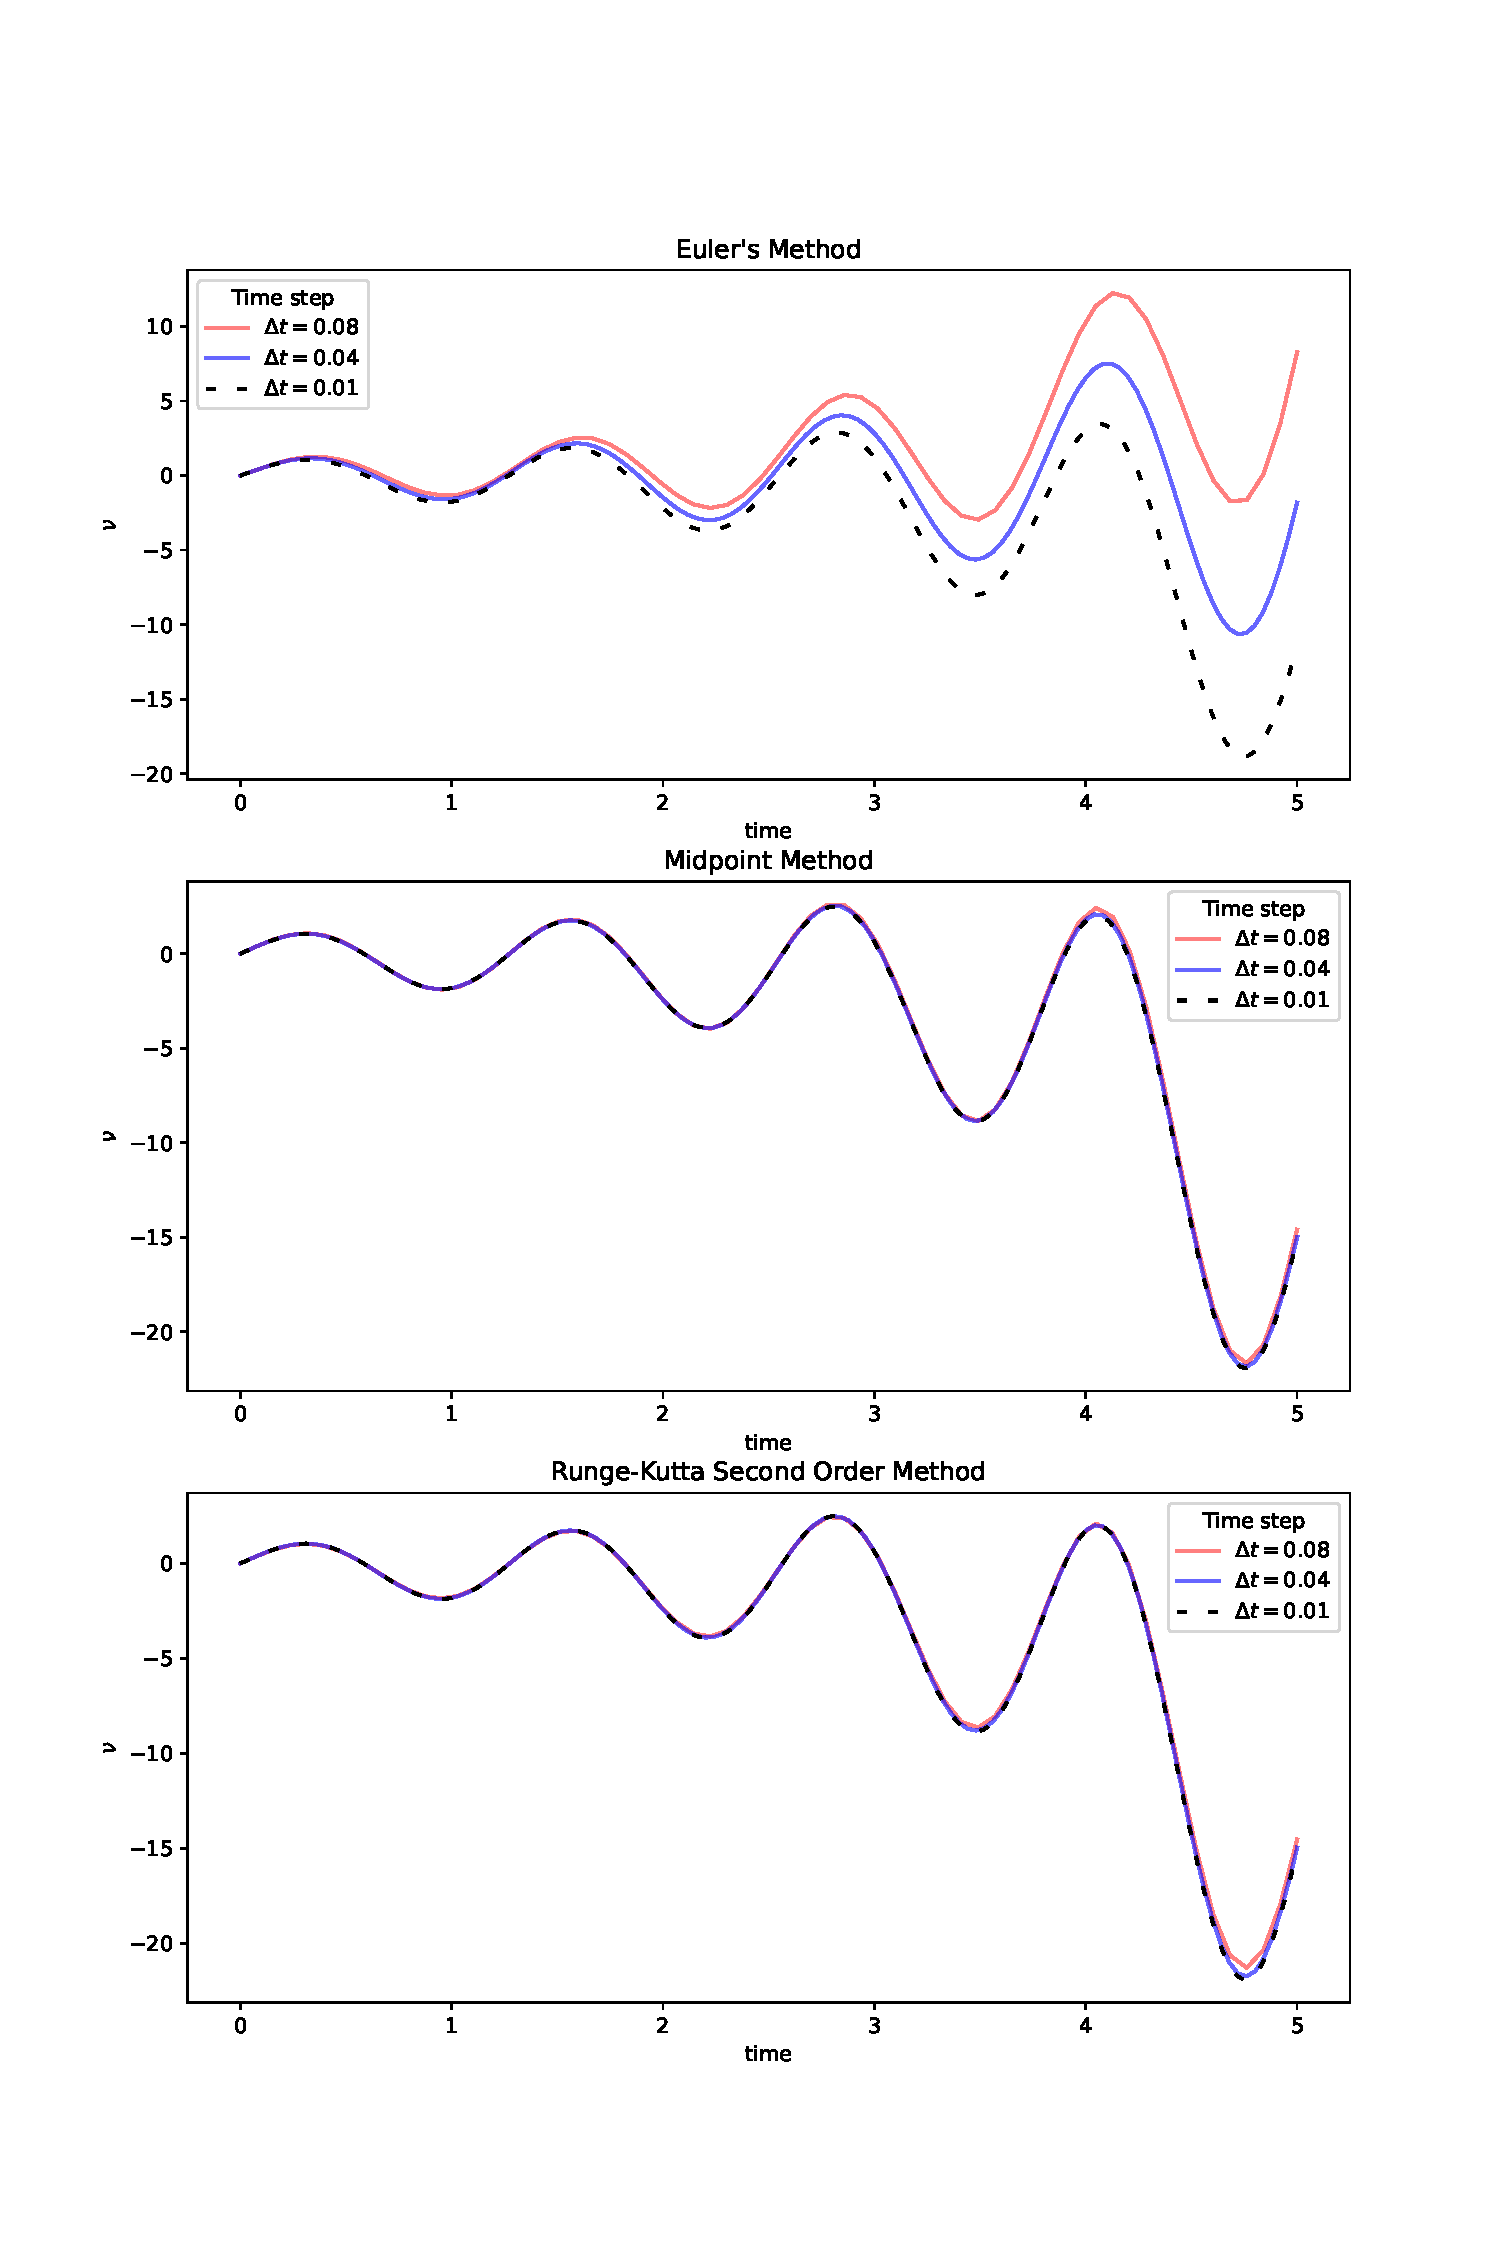
\includegraphics[scale = 0.5]{3a.pdf}
\end{figure}

\end{document}
